\documentclass{article}
\usepackage{fancyhdr}
\usepackage{titlesec}
\usepackage{graphicx}
\graphicspath{ {./img/} }

\pagestyle{fancy}
\fancyhf{}
\lhead{Modul 1 Praktikum Jaringan Komputer}
\rfoot{\footnotesize Page \thepage}
\lfoot{\footnotesize Mahyus Ihsan, S.Si, M.Si \newline Jurusan Informatika Universitas Syiah Kuala \newline Modul oleh : Diky Wahyudi, Furqan Al Ghifari, Rendika Rahmaturrizki}
\renewcommand{\headrulewidth}{1pt}
\renewcommand{\footrulewidth}{1pt}

\titleformat*{\section}{\small\bfseries}

\begin{document}
    \begin{center}  
        \textbf{Modul Praktikum Jaringan Komputer}

        \textbf{Perkenalan Jaringan Komputer}
    \end{center}

    \section*{Deskripsi Singkat}
    Praktikum Jaringan Komputer adalah praktikum untuk menunjang mata kuliah Jaringan Komputer.
    Praktikum ini menggunakan software penunjang yaitu Cisco Packet Tracer yang dapat di download langsung dari akun netacad.
    Materi praktikum akan berisi tutorial, latihan dan soal.
   

    \section*{Tujuan}
    \begin{enumerate}
        \item Dapat melakukan instalasi Cisco Packet Tracer
        \item Dapat menggunakan Cisco Packet Tracer untuk simulasi jaringan
    \end{enumerate}

    \begin{flushleft}
        \textbf{Materi 1 - Instalasi Cisco Packet Tracer}
        \newline

        Berikut adalah cara untuk melakukan instalasi Cisco Packet Tracer

        \begin{enumerate}
            \item{
                Login ke dalam akun netacad , jika belum memiliki akun silahkan untuk membuat akun terlebih dahulu. 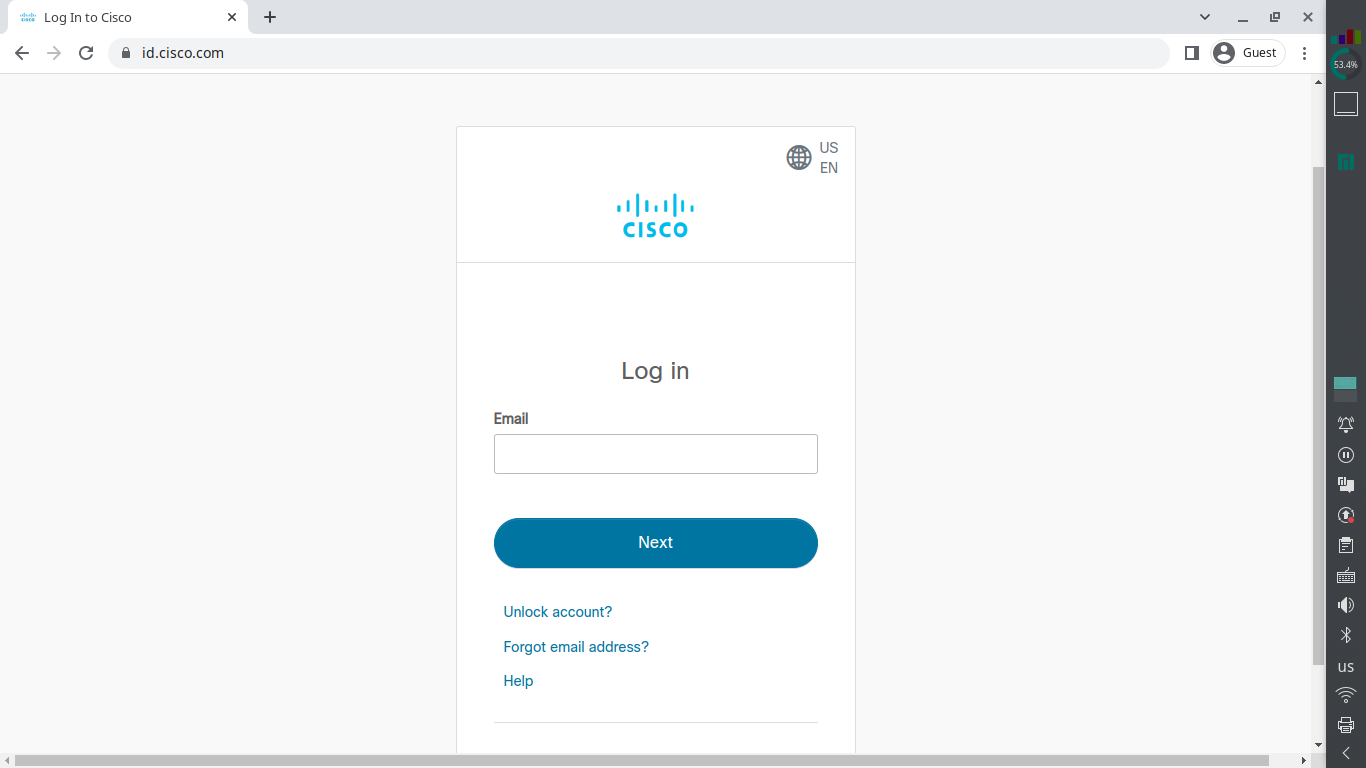
\includegraphics[scale=0.30]{login.png}
                \newline
            }
            \item{
                Jika Sudah login silahkan pilih menu \textbf{Resources - Download Packet Tracer}. 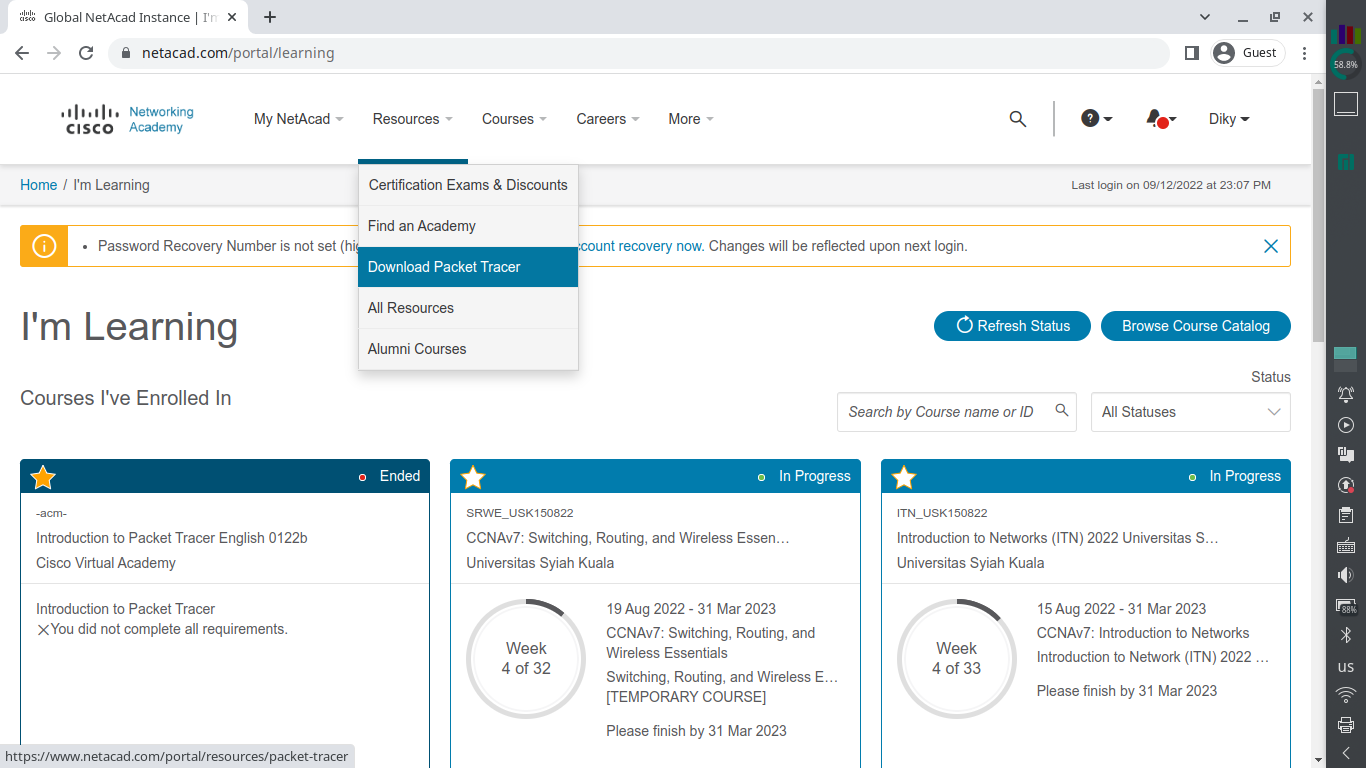
\includegraphics[scale=0.30]{dl-menu.png}
                \newline
            }
            \item{
                Lalu pilih Packet Tracer sesuai dengan sistem operasi yang digunakan. Didalam tutorial ini menggukan sistem operasi Windows jadi untuk sistem operasi lain silahkan menyesuaikan.
                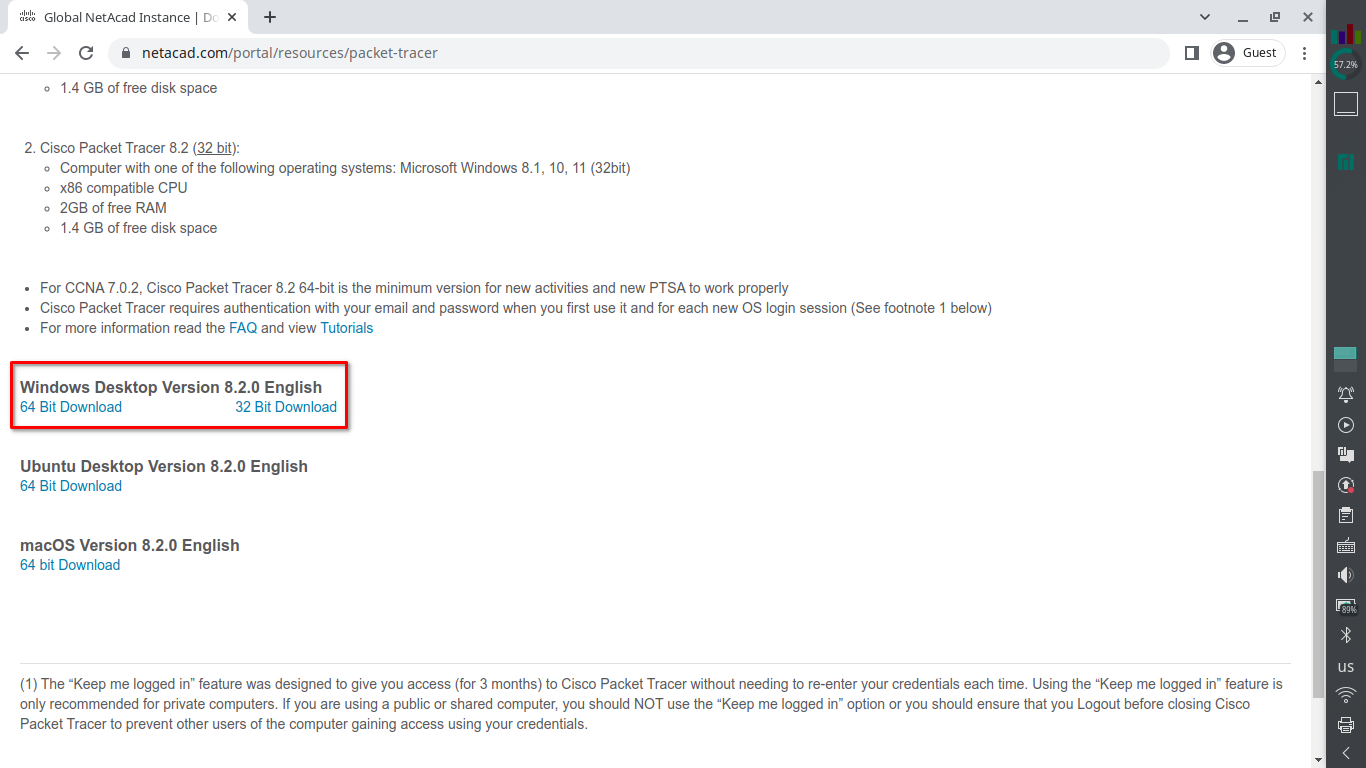
\includegraphics[scale=0.30]{dl-ver.png}
            }
            
            \item{
                Jalankan packet tracer yang telah di download tadi dan ikuti sesuai gambar berikut.
                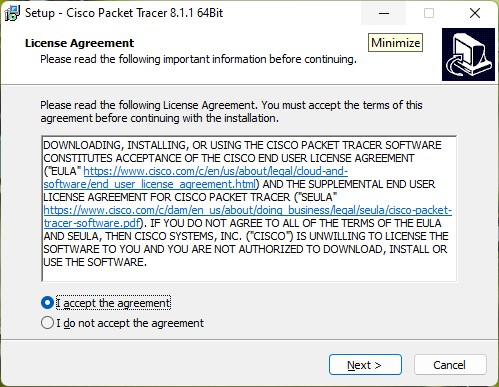
\includegraphics[scale=0.8]{install/1.jpg}
                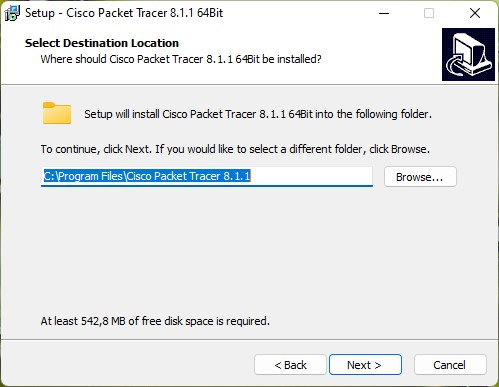
\includegraphics[scale=0.8]{install/2.jpg}
                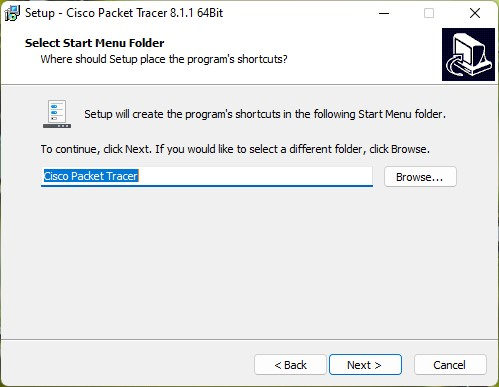
\includegraphics[scale=0.8]{install/3.jpg}
                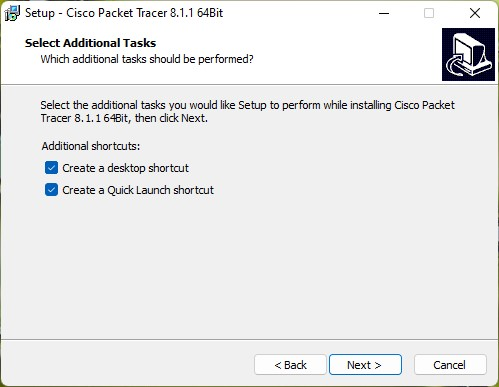
\includegraphics[scale=0.8]{install/4.jpg}
                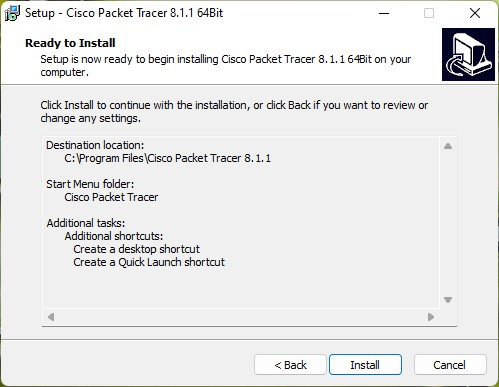
\includegraphics[scale=0.8]{install/5.jpg}
                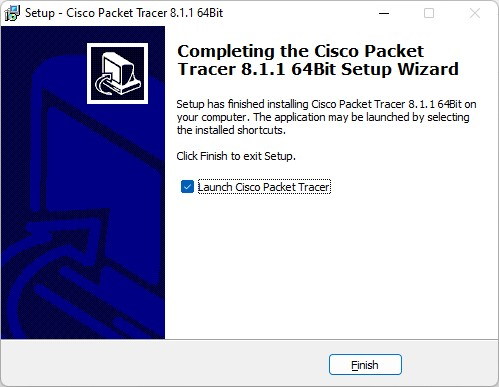
\includegraphics[scale=0.8]{install/6.jpg}
                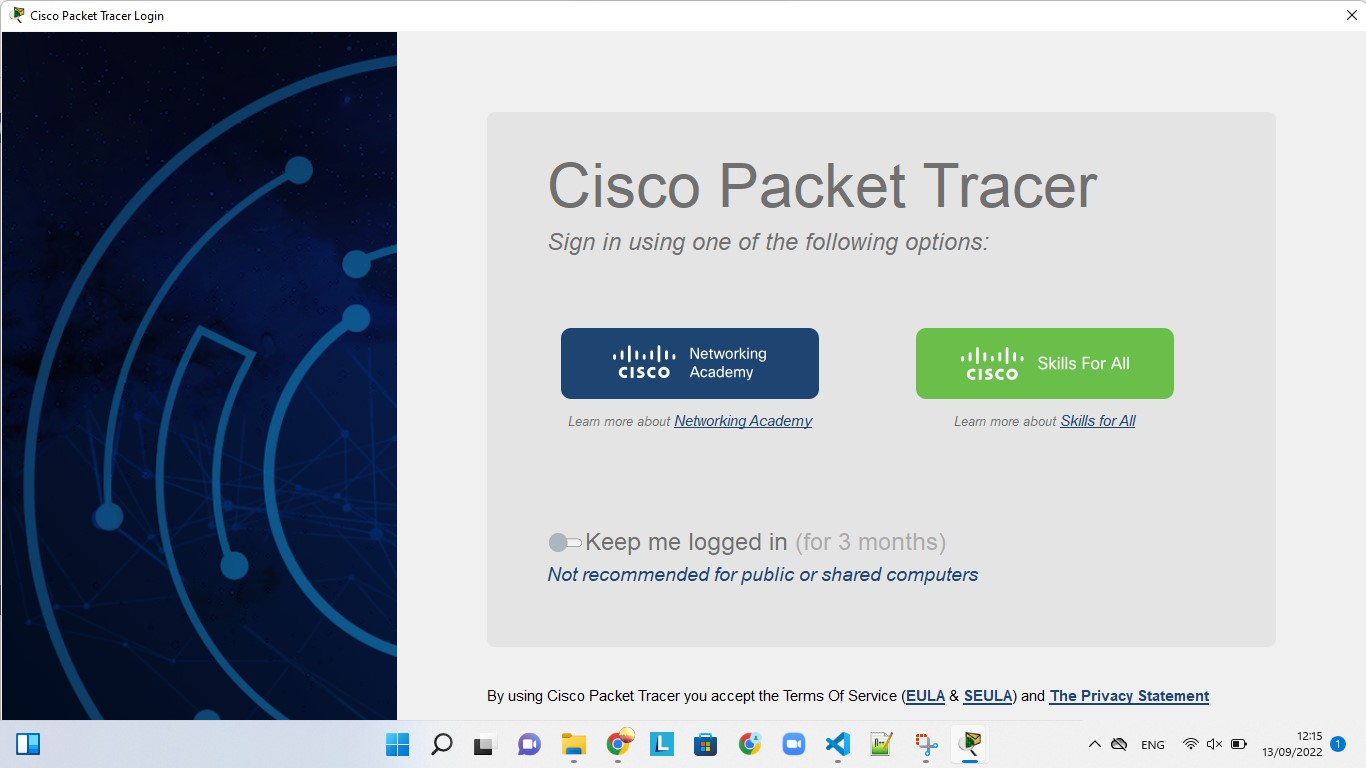
\includegraphics[scale=0.3]{install/7.jpg}
                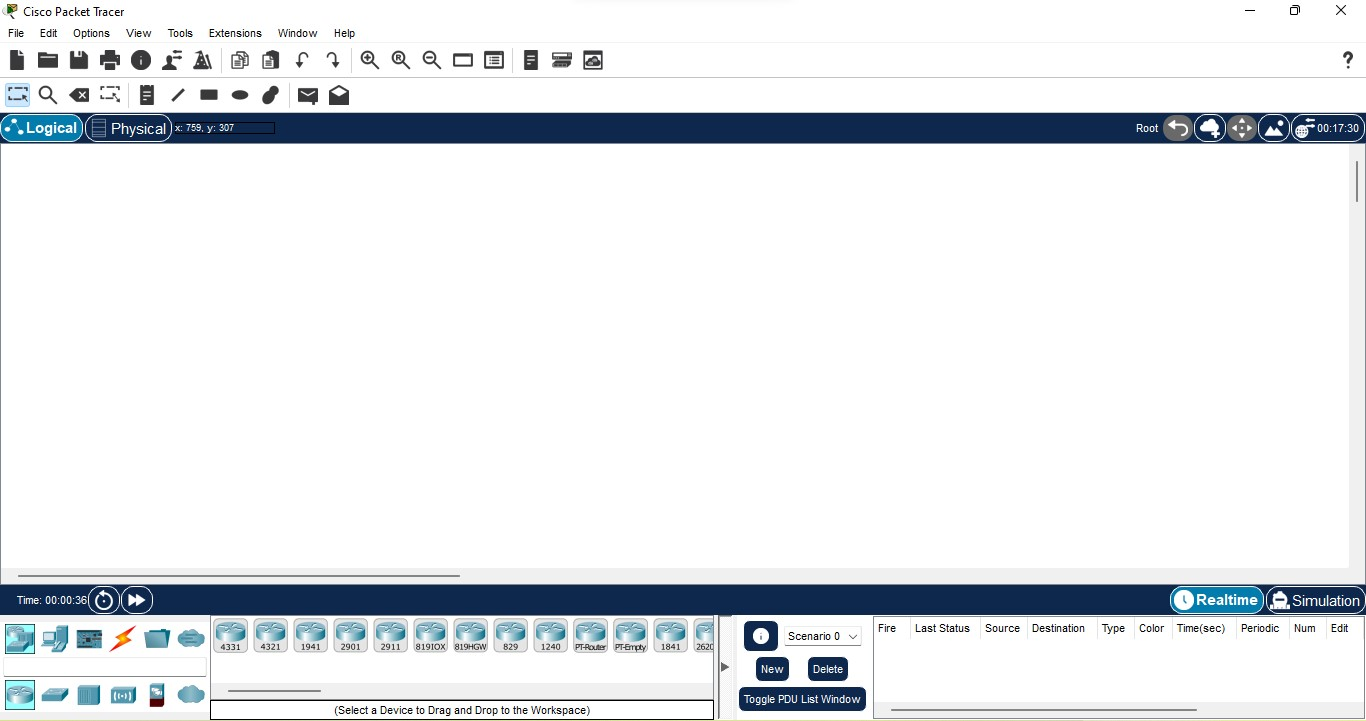
\includegraphics[scale=0.3]{install/8.jpg}
            }
        \end{enumerate}
    \end{flushleft}

    \begin{flushleft}
        \textbf{Materi 2 - End Device, Intermediate Device dan Media Transmisi}
        \newline

        \begin{enumerate}
            \setlength\itemsep{2em}

            \item \textbf{End Device}
            \begin{itemize}
                \item Desktop
                \item HP
                \item Tablet
                \item Laptop
                \item IOT Device
            \end{itemize}

            \item \textbf{Intermediate Device}
            \begin{description}
                \item[Repeater] Perangkat yang berfungsi untuk menerima sinyal yang berisi data dalam suatu jaringan. Dengan menggunakan repeater maka jangkauan jaringan akan lebih luas. 
                \item[HUB] Perangkat yang berfungsi menghubungkan banyak komputer agar dapat saling berkomunikasi dalam jaringan yang sama.
                \item[Router] Perangkat ini berfungsi meneruskan sebuah paket dari satu network pada network lain misalnya dari LAN ke WAN, atau menghubungkan antara network yang berbeda seperti LAN dihubungkan pada WAN.
                \item[Switch] Switch adalah perangkat jaringan untuk menghubungkan 2 atau lebih komputer dalam satu jaringan (concentrator).
                \item[Access Point] Access point adalah sebuah perangkat dalam jaringan komputer yang dapat menciptakan jaringan lokal nirkabel atau WLAN (Wireless Local Area Network).
                \item[Firewall Appliance] Firewall adalah sistem keamanan jaringan komputer yang mampu melindungi dari serangan virus, malware, spam, dan serangan lainnya.
            \end{description}

            \item \textbf{Media Transmisi}
            \begin{itemize}
                \item Wired
                \item Wireless
            \end{itemize}
        \end{enumerate}
    \end{flushleft}

    \begin{flushleft}
        \textbf{Materi 3 - Navigasi Switch dan Router}
        \newline

        Dalam konfigurasi switch terdapat dua mode, yang pertama adalah \textbf{User Exec Mode} dan \textbf{Privileged Exec Mode}

        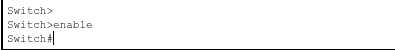
\includegraphics{switch-exec-mode.png}
        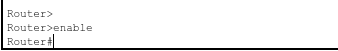
\includegraphics{router-exec-mode.png}

        \textbf{Switch$>$} atau \textbf{Router$>$} adalah \textbf{User Exec Mode}. Mode ini hanya bisa mengakses beberapa perintah saja dan fungsinya lebih ke arah \textit{view-only} untuk melakukan monitoring.
        \newline

        Sedangkan \textbf{Switch\#} atau \textbf{Router\#} adalah \textbf{Privileged EXEC Mode}. Mode ini dapat mengkases semua perintah di dalam switch dan router. Mode ini berfungsi untuk melakukan monitoring dan konfigurasi switch atau router.
        \newline

        Berikut adalah beberapa perintah yang digunakan dalam navigasi dalam IOS Cisco pada switch maupun router : 
        \begin{description}
            \item[enable] adalah perintah untuk masuk ke dalam \textbf{Privileged EXEC Mode}.
            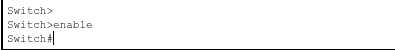
\includegraphics{switch-exec-mode.png}

            \item[disable] adalah perintah untuk kembali ke dalam \textbf{User Exec Mode}.
            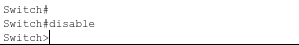
\includegraphics{disable-switch.png}

            \item[exit] adalah perintah untuk keluar dari mode saat ini dan kembali ke mode sebelumnya.
            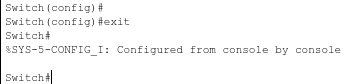
\includegraphics{exit-switch.png}

            \item[configure terminal] adalah perintah untuk masuk ke dalam mode \textbf{Global Configuration}
            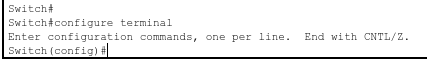
\includegraphics[scale=0.9]{conft-switch.png}

            \item[line console 0] adalah perintah untuk masuk ke dalam mode \textbf{Line Subconfiguration}
            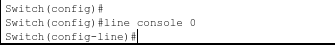
\includegraphics{line-console-switch.png}

            \item[line vty 0 15] adalah perintah untuk masuk ke dalam mode \textbf{VTY Line Subconfiguration}
            \newline
            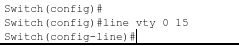
\includegraphics{vty-line-switch.png}

            \item[interface vlan 1] adalah perintah untuk masuk ke dalam mode \textbf{VLAN 1 Interface Subconfiguration}
            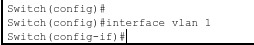
\includegraphics{vlan-switch.png}

            \item[end] adalah perintah untuk kembali ke \textbf{Privileged EXEC Mode} setelah melakukan konfigurasi.
            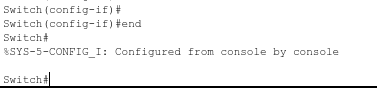
\includegraphics{end-switch.png}

            \item[show running-config] adalah perintah untuk menampilkan konfigurasi yang sedang berjalan saat ini.
            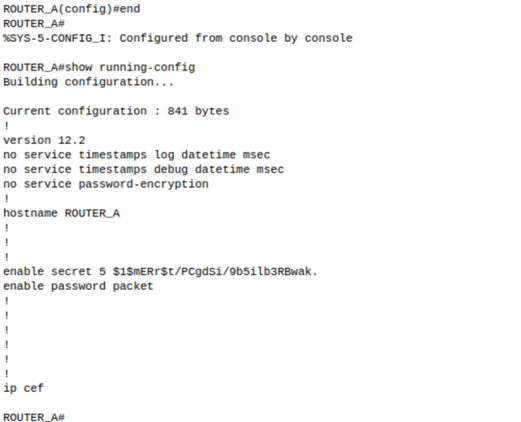
\includegraphics[scale=0.8]{running-config.png}
        \end{description}

    \end{flushleft}

    \newpage
    \begin{flushleft}
        \textbf{Tugas}
        \newline

        \begin{enumerate}
            \item Lakukan instalasi Cisco Packet Tracer pada device masing-masing, jika ada permasalahan silahkan hubungi asisten.
            \item Lakukan perintah - perintah untuk navigasi di dalam IOS Cisco pada device masing-masing.
        \end{enumerate}
    \end{flushleft}
\end{document}